% !TeX root = ..\..\main.tex
\chapter{Introduction}
\pagenumbering{arabic} %Start roman numbering

This report studies a vital financial derivative in today's markets, namely options. A standard option is a contract between two parties which gives the holder the right to buy (or sell) an asset for an agreed upon (exercise) price prior to, or on a determined (expiry) time in the future; regardless of the current (spot) price. Since the holder of the contract is not obliged to exercise the contract at the expiry time, they would not hold any liability in the absence of a price to purchase the option. The problem then becomes what is the correct price to charge the holder of the option to balance this inequality of liability. 
\nline
Whilst standard options, namely European and American style involve fixing the exercise price at the inception the option, this is not always the case with exotic options. Exotic options differ in their payment structures, expiration dates, and/or strike prices. In the case of exotic Asian style options the strike price or the spot price  

\section{A brief history of options}

The popularity of options in today's market can be easily seen by the exponential growth in their trading volume from when standardized, exchange-traded stock options were first listed in The Chicago Board Options Exchange in 1973 \cite[p. 52]{markham2002financial} to 2022, shown in \autoref{C1fig:OptionVolume}. Additionally, it is well backed up in the literature that option markets are a venue for informed trading 

\begin{figure}[H]
    \centering
    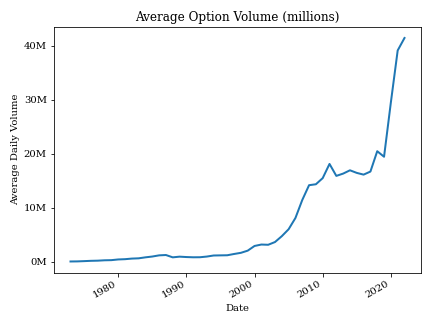
\includegraphics[width=0.65\textwidth]{Chapters/C1/plots/OptionVolume.png}
    \caption{Time series plot of the average daily option volume per annum. Data provided by the Options Clearing Corporation (OCC) \cite{THEOCC}.}
    \label{C1fig:OptionVolume}
\end{figure}

Enter some text that makes the examiner go, "wow that is a great bit of text". 

